%   % !TEX root = ../../VIII,3_Rahmen-TeX_8-1.tex
%
%
%   Band VIII, 3 N.~??S01.10
%   Signatur/Tex-Datei: LH_37_05_086-087
%   RK-Nr. 57263
%   \ref{dcc_08}
%   Überschrift: De corporum concursus scheda octava
%   Modul: Mechanik / Stoß ( )
%   Datierung: Januar 1678
%   WZ: (Bl. 87) LEd-WZ 803017 = RK-WZ 1264 (insgesamt: eins)
%   SZ:
%      \ppmH\
%      \ppmH\
%      \pleibdashv
%      \pleibvdash
%      \groesser
%         (insgesamt: 5)
%   Bilddateien (PDF): 
%      LH_37_05_086-087_d1 ((ex: lh37,5,86r)); 
%      LH_37_05_086-087_d2 ((ex: lh37,5,86v)); 
%      LH_37_05_086-087_d3 ((ex: lh37,5,87r)); 
%      LH_37_05_086-087_d4 ((ex: lh37,5,87v-1)) 
%         (insgesamt: vier)
%      getilgt: LH_37_05_086-087_d5 ((ex: lh37,5,87v-2))
%   Verzeichniseinträge: vollständig
%   \textls{} statt \textso{} (Ausnahme: Personenverzeichnis)
%
%
\selectlanguage{ngerman}%
\frenchspacing%
%
\begin{ledgroupsized}[r]{120mm}%
\footnotesize%
\pstart%
\noindent%
\textbf{Überlieferung:}%
\pend%
\end{ledgroupsized}%
\begin{ledgroupsized}[r]{114mm}%
\footnotesize%
\pstart%
\parindent -6mm%
\makebox[6mm][l]{\textit{L}}%
Konzept:
LH XXXVII~5, Bl.~86\textendash87.
Zwei Blatt 2\textsuperscript{o},
die ursprünglich wohl einen Bogen bildeten;
ein Wasserzeichen auf Bl.~87;
Papiererhaltungsmaßnahmen.
Vier vollbeschriebene Seiten,
die vom Text N.~\ref{dcc_09} %??S01\textsubscript{11} 
fortgesetzt werden;
ein Kustos am Ende von Bl.~87~v\textsuperscript{o} verweist auf die \textit{Scheda nona}. 
\pend%
%
\end{ledgroupsized}%
\begin{ledgroupsized}[r]{114mm}%
\footnotesize%
\pstart%
\parindent -6mm%
\makebox[6mm][l]{\textit{E}}%
% (tlw.)
\textsc{Fichant} 1994, S.~152\textendash158 (mit kommentierter französischer Übersetzung, S.~308\textendash316).%
\cite{01056}
\pend%
\end{ledgroupsized}%
%
\selectlanguage{latin}%
\frenchspacing%
%
\count\Bfootins=1000%
\count\Afootins=1200%
\count\Cfootins=1000
%
\vspace{8mm}%
\normalsize%
\pstart%
\noindent%
%
\lbrack86~r\textsuperscript{o}\rbrack%  %  %  %  Blatt 86r 
\hspace{46mm}
Scheda octava%
\protect\index{Sachverzeichnis}{scheda}%
\hspace{36mm}
Januar. 1678%
%
\edtext{}{%
\lemma{\textit{Unter der Überschrift, umrandet:}}\Afootnote{%
Nota bene.
Scheda octava et nona%
\protect\index{Sachverzeichnis}{scheda}
non sunt subjectae reformationi.%
\protect\index{Sachverzeichnis}{reformatio}%
\newline%
}}%
%
\edtext{}{%
\lemma{\textit{Am oberen Rand:}}\Afootnote{%
Calculus%
\protect\index{Sachverzeichnis}{calculus}
ex his\textsuperscript{[a]}
tribus principiis%
\protect\index{Sachverzeichnis}{principium calculi}%
\lbrack:\rbrack\
virium servatarum,%
\protect\index{Sachverzeichnis}{vis servata}
servatae directionis in summa,%
\protect\index{Sachverzeichnis}{directio servata in summa}
et servatarum apparentiarum.%
\protect\index{Sachverzeichnis}{apparentia servata}%
\newline\vspace{-0.4em}%
\newline%
{\footnotesize%
\textsuperscript{[a]}~his
\textit{(1)}~duobus
\textit{(2)}~tribus%
~\textit{L}%
}}}%
\pend%
\vspace{0.5em}%
%
%
\pstart%
\noindent%
Vis%
\edlabel{LH_37_05_086r_reformatio_idzg-1}
est quantitas effectus.%
\protect\index{Sachverzeichnis}{vis quantitas effectus}
Hinc vis corporis in motu existentis%
\protect\index{Sachverzeichnis}{vis corporis moti}
aestimari debet ex altitudine%
\protect\index{Sachverzeichnis}{aestimatio virium ex altitudine}%
\protect\index{Sachverzeichnis}{altitudo ascensus}
ad quam ascendere
%
\edtext{potest.
In
%
\edtext{plano inclinato \textit{AB}%
\protect\index{Sachverzeichnis}{planum inclinatum}%
}{%
\lemma{plano inclinato \textit{AB}}\Cfootnote{%
Siehe das Diagramm \lbrack\textit{Fig.~1}\rbrack\
auf S.~\pageref{LH_37_05_086r_Fig.1}.}}%
}{%
\lemma{potest.}\Bfootnote{%
\textit{(1)}~Hinc sequitur \textlangle\textendash\textrangle\
\textit{(2)}~Si duo sunt corpora mota
\textit{(3)}~\textlangle Na\textrangle\
\textit{(4)}~In plano inclinato \textit{AB}%
~\textit{L}}}
%
descendant duo globi%
\protect\index{Sachverzeichnis}{globi aequales}
%
\edtext{aequales materia%
\protect\index{Sachverzeichnis}{materia globi}
et magnitudine%
\protect\index{Sachverzeichnis}{magnitudo globi}%
}{%
\lemma{aequales}\Bfootnote{%
\hspace{-0,5mm}materia et magnitudine
\textit{erg.~L}}}
%
\textit{C} et \textit{D},
atque inde transeant sine
reflexione%
\protect\index{Sachverzeichnis}{reflexio globi}
in planum%
\protect\index{Sachverzeichnis}{planum horizontale}
%
\edtext{horizontale}{%
\lemma{horizontale}\Bfootnote{%
\textit{erg.~L}}}
%
\textit{BF}
ibique celeritatem continuent%
\protect\index{Sachverzeichnis}{celeritas continuata}%
\protect\index{Sachverzeichnis}{continuatio celeritatis}%
\lbrack;\rbrack\
patet corpora in hoc plano pervectura%
\protect\index{Sachverzeichnis}{corpus in plano perrectum}
ea celeritate,
quam in \textit{B} acquisivere.
Celeritates autem quaesitae%
\protect\index{Sachverzeichnis}{celeritas quaesita}
%
\edtext{erunt in ratione subduplicata%
\protect\index{Sachverzeichnis}{celeritas in ratione subduplicata altitudinum}%
}{%
\lemma{erunt}\Bfootnote{%
\hspace{-0,5mm}in
\textit{(1)}~quadrata
\textit{(2)}~ratione subduplicata%
~\textit{L}}}
%
altitudinum \textit{GB}, \textit{HB}
vel \textit{CB}, \textit{DB},%
\protect\index{Sachverzeichnis}{altitudo descensus}
ut constat ex
%
\edtext{demonstratis a Galilaeo.%
\protect\index{Namensregister}{\textso{Galilei} (Galilaeus, Galileus), Galileo 1564\textendash1642}%
}{%
\lemma{demonstratis a Galilaeo}\Cfootnote{% e dimostrazioni matematiche
Vgl. \textsc{G.~Galilei}, \textit{Discorsi}, giornata III, theorema II, prop. II
(Leiden 1638, S.~171\,f.;\cite{00050}
% Bologna 1656\cite{00260}, S.~130\,f.; 
\textit{GO} VIII, S.~209\,f.).\cite{00048}%
}}
%
Vires autem sunt ut altitudines%
\protect\index{Sachverzeichnis}{vis ut altitudo}
%
\edtext{\textit{CB} ad \textit{DB} sive \textit{GB} ad \textit{HB}}{%
\lemma{\textit{CB}}\Bfootnote{%
\hspace{-0,5mm}ad \textit{DB} sive \textit{GB} ad \textit{HB}
\textit{erg.~L}}}
%
ex quibus \hspace{0.3mm}corpus%
\protect\index{Sachverzeichnis}{altitudo descensus}
%
\hspace{0.3mm}\edtext{descendit
\hspace{0.3mm}seu \hspace{0.3mm}ut \hspace{0.3mm}\textit{NF} \hspace{0.3mm}ad \hspace{0.3mm}\textit{PF},
\hspace{0.3mm}vel \hspace{0.3mm}\textit{LF} \hspace{0.3mm}ad \hspace{0.3mm}\textit{MF}
\hspace{0.3mm}ad \hspace{0.3mm}quas}{%
\lemma{descendit}\Bfootnote{%
\textit{(1)}~seu
\textit{(2)}~seu ut % \textit{NF} ad 
\lbrack...\rbrack\ \textit{PF}, vel
\textit{(a)}~\textit{LM}
\textit{(b)}~\textit{LF} ad \textit{MF} ad
\textit{(aa)}~quam
\textit{(bb)}~quas%
~\textit{L}}}
%
\hspace{0.3mm}postea \hspace{0.3mm}sese \hspace{0.3mm}attollere \hspace{0.3mm}potest,%
\protect\index{Sachverzeichnis}{altitudo ascensus}
\hspace{0.3mm}quae \hspace{0.3mm}hoc \hspace{0.3mm}loco
%
\hspace{0.3mm}\edtext{\lbrack eaedem\rbrack}{%
\lemma{eadem}\Bfootnote{%
\textit{L~ändert Hrsg. nach~E, S.~153%
\cite{01056}}}}
%
\hspace{0.3mm}compendii
\pend
\newpage
  \centerline{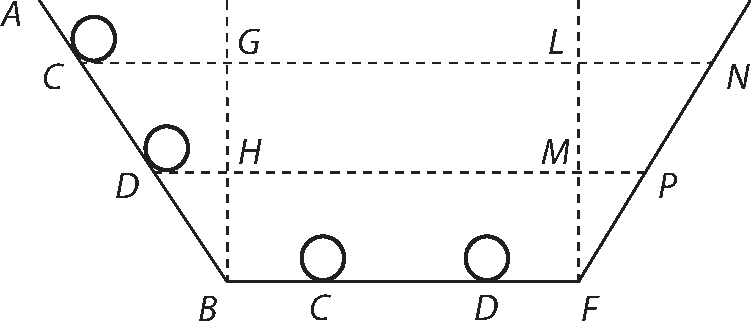
\includegraphics[width=0.56\textwidth]{gesamttex/edit_VIII,3/images/LH_37_05_086-087_d1.pdf}}%
  \vspace{0.5em}
  \centerline{\hspace{6,0mm}\lbrack\textit{Fig.~1}\rbrack}%
  \label{LH_37_05_086r_Fig.1}%
  \vspace{1.3em}%
%  \newpage%
%
%
\pstart
\noindent causa%
\protect\index{Sachverzeichnis}{compendium}
%
\edtext{\lbrack supponuntur\rbrack:}{%
\lemma{supponitur}\Bfootnote{%
\textit{L~ändert Hrsg. nach~E, S.~153%
\cite{01056}}}}
%
ergo
%
\edtext{erunt corporum duorum
ut \textit{C}, \textit{D}
etiam in horizontali plano%
\protect\index{Sachverzeichnis}{planum horizontale}
\lbrack\textit{BF}\rbrack\
motorum vires%
\protect\index{Sachverzeichnis}{vis corporis moti}
ut quadrata celeritatum.%
\protect\index{Sachverzeichnis}{vis ut quadratum celeritatis}
%
\edlabel{LH_37_05_086r_quadrataceleritatum-1}%
Hinc vis eadem manet,%
\protect\index{Sachverzeichnis}{vis eadem manens}
non quando eadem manet quantitas motus,%
\protect\index{Sachverzeichnis}{quantitas motus eadem}
seu summa factorum ex celeritatibus in corpora,%
\protect\index{Sachverzeichnis}{summa factorum ex celeritatibus in corpora}
sed summa factorum ex quadratis celeritatum in corpora.%
\protect\index{Sachverzeichnis}{summa factorum ex quadratis celeritatum}%
\protect\index{Sachverzeichnis}{quadratum celeritatis}%
\edlabel{LH_37_05_086r_reformatio_idzg-2}%
\edlabel{LH_37_05_086r_quadrataceleritatum-2}%
}{%
\lemma{erunt}\Bfootnote{%
\textit{(1)}~corpora ejus
\textit{(2)}~corporis
\textit{(3)}~corporum
\textit{(a)}~duorum aequalium vires ut quadrata celeritatum. Hinc
\textit{(b)}~duorum ut % \textit{C}, \textit{D} etiam in 
\lbrack...\rbrack\ horizontali plano
\textbar~\textit{BM} \textit{ändert Hrsg.}~%
\textbar\ motorum vires % ut quadrata 
\lbrack...\rbrack\ celeritatum. Hinc
\textit{(aa)}~non
\textit{(bb)}~vis eadem % manet, non quando eadem manet 
\lbrack...\rbrack\ quantitas motus,
\textit{(aaa)}~sed quando eadem manet quanti
\textit{(bbb)}~seu summa % factorum ex celeritatibus in corpora, sed summa factorum ex quadratis celeritatum 
\lbrack...\rbrack\ in corpora.%
~\textit{L}}}%
\pend
\pstart%
Sint corpora \textit{a} \textit{b},
eorum celeritates
$\displaystyle\efrac{\textup{ante}}{\textup{post}}$
concursum%
\protect\index{Sachverzeichnis}{celeritas post concursum}
$\displaystyle\efrac{e \ i}{\epsilon \ y}$
\edlabel{LH_37_05_086r_aequatioinfall-1}%
fiet aequatio infallibilis%
\protect\index{Sachverzeichnis}{aequatio infallibilis}
$a\,e^2 + b\,i^2$
aequ.
$a\,\epsilon^2 + b\,y^2,$
vel
$a\,e^2 - a\,\epsilon^2$
aequ.
$b\,y^2 - b\,i^2,$
seu
$\displaystyle \frac{a}{b}$
aequ.
$\displaystyle \frac{y^2 - i^2}{e^2 - \epsilon^2},$
vel
$\displaystyle \frac{a}{b}$
aequ.
$\displaystyle \frac{y+i,\;y-i}{e+\epsilon,\;e-\epsilon}.$%
\edlabel{LH_37_05_086r_aequatioinfall-2}
%
\edtext{Hinc corollarium:%
\protect\index{Sachverzeichnis}{corollarium}
si \textit{y} major quam \textit{i},
erit $\displaystyle \epsilon$ minor quam \textit{e}.}{%
\lemma{Hinc}\Bfootnote{%
\hspace{-0,5mm}corollarium \lbrack...\rbrack\ quam \textit{e}.
\textit{erg.~L}}}%
\rule[-5mm]{0mm}{11mm}
%
\pend%
%
\pstart%
Porro%
\edlabel{LH_37_05_086r_percussioeadem-1}
uti vis absoluta%
\protect\index{Sachverzeichnis}{vis absoluta}
manere debet eadem,%
\protect\index{Sachverzeichnis}{vis eadem manens}
ita et eadem manere debet vis respectiva,%
\protect\index{Sachverzeichnis}{vis respectiva}
id est%
\lbrack:\rbrack\
%
\edtext{quemadmodum % \lbrack,\rbrack\
relatione ad totum systema habita%
\protect\index{Sachverzeichnis}{relatio ad systema}%
\protect\index{Sachverzeichnis}{systema}% \lbrack,\rbrack\
}{%
\lemma{quemadmodum}\Bfootnote{%
\textit{(1)}~in syste
\textit{(2)}~relatione ad totum systema habita%
~\textit{L}}}
%
semper corpus facultatem%
\protect\index{Sachverzeichnis}{facultas assurgendi}
habere debet
(\protect\vphantom)%
nisi quid impediat%
\protect\vphantom()
in tantum rursus assurgendi supra horizontem%
\protect\index{Sachverzeichnis}{horizon}
seu recedendi a terra,%
\protect\index{Sachverzeichnis}{terra}%
\protect\index{Sachverzeichnis}{recessus a terra}
in quantum ad terram
%
\edtext{accessit%
\protect\index{Sachverzeichnis}{accessus ad terram}%
\protect\index{Sachverzeichnis}{terra}
et quidem eodem tempore,
si omnia requisita adsint;
ita etiam corpora duo
vim habere debent ab ictu%
\protect\index{Sachverzeichnis}{vis ab ictu}}{%
\lemma{accessit}\Bfootnote{%
\textit{(1)}~ita etiam
\textit{(2)}~et quidem % eodem tempore, si omnia requisita adsint;
\lbrack...\rbrack\ ita etiam
\textit{(1)}~corpus quod in aliud corpus impegit
\textit{(2)}~corpora duo % vim habere debent 
\lbrack...\rbrack\ ab ictu%
~\textit{L}}}
%
in tantum a se invicem recedendi%
\protect\index{Sachverzeichnis}{vis corporum a se invicem recedendi}
in quantum sibi accessere.
%
\edlabel{LH_37_05_086r_percussioeadem-3}%
Accedit ratio,%
\protect\index{Sachverzeichnis}{ratio}
quod omnia eodem modo debent
%
\edtext{apparere,
in uno corporum concurrentium existenti,%
\protect\index{Sachverzeichnis}{corpora concurrentia}
sive}{%
\lemma{apparere,}\Bfootnote{%
\textit{(1)}~in u
\textit{(2)}~sive in
\textit{(3)}~in uno % corporum concurrentium 
\lbrack...\rbrack\ existenti, sive
~\textit{L}}}
%
ipse in moto aut quiescente exi\-stat% ,%
\protect\index{Sachverzeichnis}{corpus motum}%
\protect\index{Sachverzeichnis}{corpus quiescens}%
\lbrack:\rbrack\
ex.~gr. idem eventus%
\protect\index{Sachverzeichnis}{eventus}
ei debet apparere,
sive ipse in murum incurrat%
\protect\index{Sachverzeichnis}{incursus in murum}
sive murus in ipsum.%
\protect\index{Sachverzeichnis}{murus}
Cum enim causam%
\protect\index{Sachverzeichnis}{causa discreta}
nulla ratione discernere possit,%
\protect\index{Sachverzeichnis}{ratio}
etiamsi vel angelicam sapientiam%
\protect\index{Sachverzeichnis}{sapientia angelica}
%
\edtext{haberet,
nec}{%
\lemma{haberet,}\Bfootnote{%
\textit{(1)}~tamen
\textit{(2)}~nec%
~\textit{L}}}
%
effectum discernere posse debet.%
\protect\index{Sachverzeichnis}{effectus discretus}
Erit ergo semper et percussio eadem,%
\protect\index{Sachverzeichnis}{percussio}
et idem conatus separationis.%
\protect\index{Sachverzeichnis}{conatus separationis}%
\edlabel{LH_37_05_086r_percussioeadem-2}%
%
\pend%
%
\pstart%
Hinc si duo corpora concurrant%
\protect\index{Sachverzeichnis}{corpora concurrentia}
%
\edtext{utcunque,
tunc ante concursum
vel post concursum%
\protect\index{Sachverzeichnis}{concursus corporum}
in easdem tendunt partes
vel in diversas.}{%
\lemma{utcunque,}\Bfootnote{%
\textit{(1)}~tunc vel post concursum in easdem tendunt partes vel in diversas, si in
\textit{(a)}~easdem
\textit{(b)}~diversas tunc
\textit{(aa)}~summa celerita
\textit{(bb)}~ut distantia maneat eadem eodem tempore ante et post concursum, necesse est esse
\textit{(2)}~tunc ante \lbrack...\rbrack\ in diversas.%
~\textit{L}}}
%
Si in easdem tendunt partes,%
\protect\index{Sachverzeichnis}{corpora in easdem partes tendentia}
tunc erit distantia celeritatum differentia.%
\protect\index{Sachverzeichnis}{distantia corporum ut differentia celeritatum}
Si in
%
\edtext{\lbrack diversas\rbrack,%
\protect\index{Sachverzeichnis}{corpora in diversas partes tendentia}}{%
\lemma{easdem}\Bfootnote{%
\textit{L~ändert Hrsg. nach~E, S.~153%
\cite{01056}}}}
%
summa,%
\protect\index{Sachverzeichnis}{distantia corporum ut summa celeritatum}
seu erit:
$\ppmG e\; \ppmH i\ \text{aequ.}\ (\ppmG\!)\, \epsilon\; (\ppmH\!)\, y.$
Quae signa ut explicentur,%
\protect\index{Sachverzeichnis}{signum explicandum}
hoc considerandum est:
%
\lbrack86~v\textsuperscript{o}\rbrack\ %  %  %  %  Blatt 86v
%
\pend%
%
\pstart%
Si corpora in easdem tendunt partes,%
\protect\index{Sachverzeichnis}{corpora in easdem partes tendentia}
et id quod assequitur aliud tardius antecedens,%
\protect\index{Sachverzeichnis}{corpus antecedens tardius}
ipso antecedente majus est,%
\protect\index{Sachverzeichnis}{corpus assequens majus}
tunc post concursum%
\protect\index{Sachverzeichnis}{concursus corporum}
ambo tendunt in easdem partes,
adeoque eo casu
%
\edtext{fit $e - i$ aequ. $y - \epsilon.$}{%
\lemma{fit}\Bfootnote{%
\textit{(1)}~$e + i$ aequ. $\epsilon + y.$
\textit{(2)}~$e - i$ aequ. $y - \epsilon.$%
~\textit{L}}}
\pend%
%
\pstart%
Si vero corpora tendunt in easdem partes,%
\protect\index{Sachverzeichnis}{corpora in easdem partes tendentia}
et id quod alterum assequitur eo minus est,%
\protect\index{Sachverzeichnis}{corpus assequens minus}
tunc repellitur,%
\protect\index{Sachverzeichnis}{corpus assequens repulsum}
et fit $e - i$ aequ. $\epsilon + y.$
\pend%
%
\pstart%
Si corpora tendunt in partes contrarias,%
\protect\index{Sachverzeichnis}{corpora in partes contrarias tendentia}
tunc si unum est majus et celerius,%
\protect\index{Sachverzeichnis}{corpus majus et celerius}
alterum minus et tardius,%
\protect\index{Sachverzeichnis}{corpus minus et tardius}
et majus ac celerius ponatur esse \textit{a},
tunc fiet:
%
\edtext{$e-i,$ aequ. $y - \epsilon.$}{%
{\lemma{\textit{Am Rand:}}\Afootnote{%
Imo error.%
\protect\index{Sachverzeichnis}{error}%
%\textsuperscript{\lbrack a\rbrack}%
%\newline%
%\newline%
%{\footnotesize%
%\textsuperscript{\lbrack a\rbrack}~%
%Richtig wäre tatsächlich:
%$e + i = y - \epsilon.$
%Siehe \textsc{Fichant} 1994, S.~310, Anm.~4.%
%\cite{01056}%
%}
}}%
{\lemma{$e-i,$ aequ. $y - \epsilon$}\Cfootnote{%
Die Aussage ist, wie Leibniz in der hierauf bezogenen Randbemerkung festhält, falsch.
Richtig wäre: $e + i = y - \epsilon.$
Vgl. S.~\refpassage{LH_37_05_087v_eskfz-1}{LH_37_05_087v_eskfz-3}.
Siehe zudem \textsc{Fichant} 1994, S.~310, Anm.~4.%
\cite{01056}%
}}%
}
\pend%
%
\pstart%
Si%
\edlabel{LH_37_05_086v_cidcamp-1}
corpora tendunt in partes contrarias,%
\protect\index{Sachverzeichnis}{corpora in partes contrarias tendentia}
tunc id
quod est minus%
\protect\index{Sachverzeichnis}{corpus minus repulsum}
semper repelletur,
quantacunque celeritate%
\protect\index{Sachverzeichnis}{celeritas corporis minoris}
%
\edtext{feratur,
seu quantamcunque vim habeat.%
\protect\index{Sachverzeichnis}{vis corporis minoris}
Nam}{%
\lemma{feratur}\Bfootnote{%
\textit{(1)}~. Si corpora tendunt in partes contrarias, tunc
\textit{(2)}~, seu quantamcunque vim habeat. Nam%
~\textit{L}}}
%
cum repellatur
si incurrat in majus quiescens,%
\protect\index{Sachverzeichnis}{corpus majus quiescens}
multo magis repelletur%
\protect\index{Sachverzeichnis}{corpus minus repulsum}
si incurrat in majus
%
\edlabel{LH_37_05_086v_berh-1}%
occurrens.%
\protect\index{Sachverzeichnis}{corpus majus occurrens}%
\edlabel{LH_37_05_086v_cidcamp-2}%
%
\edtext{}{%
{\xxref{LH_37_05_086v_berh-1}{LH_37_05_086v_berh-2}}%
{\lemma{occurrens.}\Bfootnote{%
\textit{(1)}~Corpus majus repelli
\textit{(2)}~Posito quod % centrum gravitatis in easdem semper tendat 
\lbrack...\rbrack\ partes, sequitur
\textit{(a)}~corpus
\textit{(b)}~corpora ambo repelli 
\textit{(aa)}~cum aequali
\textit{(bb)}~cum celeritate concurrunt reciproca magnitudini.%
~\textit{L}}}}%
%
\pend%
%
\pstart%
Posito%
\edlabel{LH_37_05_086v_velorecipr-1}
quod centrum gravitatis%
\protect\index{Sachverzeichnis}{centrum gravitatis in easdem partes tendens}
in easdem semper tendat partes,
sequitur corpora ambo repelli%
\protect\index{Sachverzeichnis}{corpora ambo repulsa}
cum celeritate concurrunt reciproca magnitudini.%
\protect\index{Sachverzeichnis}{celeritas concursus reciproca magnitudini}%
\edlabel{LH_37_05_086v_berh-2}
Tunc enim centrum gravitatis quiescit.%
\edlabel{LH_37_05_086v_velorecipr-2}%
\protect\index{Sachverzeichnis}{centrum gravitatis quiescens}
\pend%
%\newpage%
%
\pstart%
Hinc si corpus majus incurrat in minus occurrens%
\protect\index{Sachverzeichnis}{corpus majus occurrens}%
\protect\index{Sachverzeichnis}{corpus incurrens}%
\protect\index{Sachverzeichnis}{corpus occurrens}
et major
%
\edtext{sit celeritas minoris%
\protect\index{Sachverzeichnis}{celeritas corporis minoris}
quam in \hspace{0.3mm}reciproca}{%
\lemma{sit}\Bfootnote{%
\textit{(1)}~celeritat\textlangle e\textrangle\
\textit{(2)}~celeritas minoris quam
\textit{(a)}~reciproca
\textit{(b)}~in reciproca%
~\textit{L}}}
%
\hspace{0.3mm}magnitudinum \hspace{0.3mm}ratione,%
\protect\index{Sachverzeichnis}{ratio magnitudinum reciproca}
\hspace{0.3mm}ambo \hspace{0.3mm}repellentur% ; %
\protect\index{Sachverzeichnis}{corpora ambo repulsa}%
\lbrack:\rbrack\
\hspace{0.3mm}minus \hspace{0.3mm}vel \hspace{0.3mm}ideo
\hspace{0.3mm}quia \hspace{0.3mm}minus \hspace{0.3mm}est,
\pend
\newpage
  \centerline{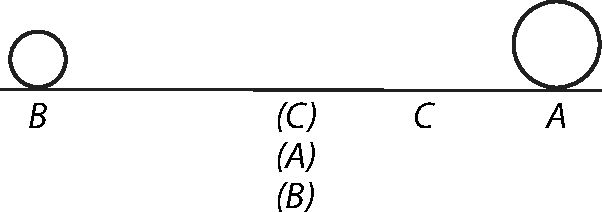
\includegraphics[width=0.44\textwidth]{gesamttex/edit_VIII,3/images/LH_37_05_086-087_d2.pdf}}%\hspace{50mm}
  \vspace{0.5em}
  \centerline{\lbrack\textit{Fig.~2}\rbrack}%\hspace{48mm}
%  \label{LH_37_05_086v_Fig.2}%
  \vspace{1.1em}%
 % \newpage%
%
%
\pstart
\noindent
majus vero,
quia
%
\edtext{ex praecedenti}{%
\lemma{ex praecedenti}\Cfootnote{%
Vgl. S.~\refpassage{LH_37_05_086v_velorecipr-1}{LH_37_05_086v_velorecipr-2}.}}%
%ex: LH_37_05_086v_cidcamp-
\lbrack,\rbrack\
%
etiam cum minori vi occurreret alterum%
\lbrack,\rbrack\
repellebatur.
Hinc eo casu erit%
\protect\index{Sachverzeichnis}{casus}
\edtext{$i-e \ \text{aequ.} \ \epsilon + y.$}{%
\lemma{$i-e \ \text{aequ.} \ \epsilon + y$}\Cfootnote{%
%Auch diese Aussage ist falsch.
Richtig wäre vielmehr: $e + i = \epsilon + y.$
Vgl. S.~\refpassage{LH_37_05_087v_eskfz-1}{LH_37_05_087v_eskfz-3}.
Siehe zudem \textsc{Fichant} 1994, S.~311, Anm.~1.%
\cite{01056}%
}}
\pend%
%
\pstart%
Videri
%
\edtext{alicui}{%
\lemma{alicui}\Cfootnote{%
Siehe etwa N.~\ref{dcc_03},
S.~\refpassage{LH_35_09_23_008v_rcprdpl-1}{LH_35_09_23_008v_rcprdpl-2}.%
}}
%
possit verum hoc theorema:%
\protect\index{Sachverzeichnis}{theorema}
%
\edtext{si corpus}{%
\lemma{si}\Bfootnote{\hspace{-0,5mm}%
\textbar~majus \textit{gestr.}~%
\textbar\ corpus%
\textit{L}}}
%
incurrat alteri occurrenti,%
\protect\index{Sachverzeichnis}{corpus incurrens occurrenti}
celeritate duplo majore quam reciproca,%
\protect\index{Sachverzeichnis}{celeritas reciproca}%
\protect\index{Sachverzeichnis}{celeritas duplo major quam reciproca}
quiescet;%
\protect\index{Sachverzeichnis}{corpus quiescens}
nam ob reciprocam conabitur
%
\edtext{redire via illa%
\protect\index{Sachverzeichnis}{conatus redeundi}
qua venit,
et illa reciproca celeritate%
\protect\index{Sachverzeichnis}{celeritas reciproca}%
\lbrack;\rbrack}{%
\lemma{redire}\Bfootnote{%
\textit{(1)}~ea qua venit
\textit{(2)}~via
\textit{(a)}~, et celeritate
\textit{(b)}~illa qua % venit, et illa 
\lbrack...\rbrack\ reciproca celeritate%
~\textit{L}}}
%
sed altera parte celeritatis
eodem conatu tentat pergere,%
\protect\index{Sachverzeichnis}{conatus pergendi}
ergo quiesceret%
\protect\index{Sachverzeichnis}{corpus quiescens}%
\lbrack;\rbrack\
hinc sequeretur
minus incurrens in majus occurrens%
\protect\index{Sachverzeichnis}{corpus minus occurrens}%
\protect\index{Sachverzeichnis}{corpus incurrens}%
\protect\index{Sachverzeichnis}{corpus occurrens}
aliquando non repelli,%
\protect\index{Sachverzeichnis}{corpus repulsum}
quod puto
%
\edtext{ex prioribus}{%
\lemma{ex prioribus}\Cfootnote{%
Vgl. S.~\refpassage{LH_37_05_086v_cidcamp-1}{LH_37_05_086v_cidcamp-2}.}}
%
absurdum.%
\protect\index{Sachverzeichnis}{absurdum}
An vero hoc theorema%
\protect\index{Sachverzeichnis}{theorema}
in majori non habeat locum,
inquirendum.
\pend%
%
\pstart%
\label{LH_37_05_086v_vaikea}%
Si majus occurrat minori,%
\protect\index{Sachverzeichnis}{corpus majus occurrens}
fieri potest
ut majus repellatur,%
\protect\index{Sachverzeichnis}{corpus majus repulsum}
fieri etiam potest
ut majus progrediatur,%
\protect\index{Sachverzeichnis}{corpus majus progrediens}
ergo etiam fieri potest
ut quiescat.%
\protect\index{Sachverzeichnis}{corpus majus quiescens}
Quando autem quiescit majus,%
\protect\index{Sachverzeichnis}{corpus majus quiescens}
tunc via corporis minoris repulsi aequatur%
\protect\index{Sachverzeichnis}{via corporis minoris repulsi}%
\protect\index{Sachverzeichnis}{corpus minus repulsum}
viae centri gravitatis ante concursum%
\protect\index{Sachverzeichnis}{via centri gravitatis ante concursum}%
\lbrack,\rbrack\
%
\edtext{posito
\lbrack hoc\rbrack\
semper eodem modo procedere%
\lbrack;\rbrack}{%
\lemma{posito}\Bfootnote{\hspace{-0,5mm}%
\textbar~hoc \textit{erg. Hrsg.}%
\textbar\ semper eodem modo procedere
\textit{erg.~L}}}
%
via autem centri gravitatis%
\protect\index{Sachverzeichnis}{via centri gravitatis in occursu}%
\protect\index{Sachverzeichnis}{centrum gravitatis}
duobus corporibus sibi occurrentibus%
\protect\index{Sachverzeichnis}{corpora sibi occurrentia}
sic investigabitur:
\pend%
\pstart%
\noindent%
\textit{AC} aequ.
$\displaystyle \frac{b}{a+b}\,\overline{e+i}$
et \textit{BC} aequ.
$\displaystyle \frac{a}{a+b}\,\overline{e+i}.$%
\edlabel{LH_37_05_086v_wsytp-1}%
%
\edtext{}{%
{\xxref{LH_37_05_086v_wsytp-1}{LH_37_05_086v_wsytp-2}}%
{\lemma{$\displaystyle \frac{a}{a+b}\,\overline{e+i}.$}\Bfootnote{%
\textit{(1)}~Si corpus \textit{A} majorem
\textit{(2)}~Corpus quod majorem%
~\textit{L}}}}
%
%\pend%
%%
%\pstart%
\edtext{}{{\xxref{KZeitz103}{KZeitz104}}%
{%
\lemma{\textit{Am Rand:}}\Afootnote{%
\textit{A} et \textit{C} tendunt in easdem partes.%
\protect\index{Sachverzeichnis}{corpora in easdem partes tendentia}
\textit{A(C)} aequ. \textit{e}.
\textit{AC} aequ. $\displaystyle \frac{b}{a+b}\lbrack\overline{e + i}\rbrack\textsuperscript{\lbrack a\rbrack}.$
\newline\vspace{-0.4em}%
\newline%
{\footnotesize%
\textsuperscript{\lbrack a\rbrack}~%
$\displaystyle\overline{e + i}$
\textit{erg. Hrsg.}\vspace{-4mm}}}}}%
Corpus\edlabel{KZeitz103} quod majorem%
\protect\index{Sachverzeichnis}{celeritas major quam reciproca magnitudini}%
\edlabel{LH_37_05_086v_wsytp-2}
%
quam reciprocam magnitudini%
\protect\index{Sachverzeichnis}{magnitudo corporis occurrentis}
alterius celeritatem habet,%
\protect\index{Sachverzeichnis}{celeritas reciproca magnitudini}%
\protect\index{Sachverzeichnis}{celeritas major quam reciproca magnitudini}
in eandem tendit partem
cum centro gravitatis%
\lbrack:\rbrack\
nam cum reciprocam habet%
\protect\index{Sachverzeichnis}{celeritas reciproca magnitudini}%
\lbrack,\rbrack\
quiescit
%
\edtext{centrum,%
\protect\index{Sachverzeichnis}{centrum gravitatis quiescens}%
}{%
\lemma{centrum}\Bfootnote{%
\textit{erg.~L}}}
%
major ergo%
\protect\index{Sachverzeichnis}{celeritas major quam reciproca magnitudini}
quae ipsi%
\lbrack,\rbrack\
caeteris ut prius manentibus%
\lbrack,\rbrack\
additur in aliquam partem
celeritas
facit centrum illuc ire.%
\protect\index{Sachverzeichnis}{centrum gravitatis motum}\edlabel{KZeitz104}%%
\pend%
\newpage
%\vspace{0.5em}%
%
\pstart%
\noindent%
\lbrack\textit{Nachfolgend kleingedruckter Text in L gestrichen:}\rbrack 
\pend%
\vspace{0.5em}%
%
\footnotesize%
\pstart%
\noindent%
Sit ergo $ae \ \groesser \ bi.$
Cadet \textit{C} inter $\underset{\displaystyle \textit{(A)}}{\textit{(C)}}$ et \textit{A},
adeoque fiet 
\textit{C(C)} aequ. \textit{A(A)} $-$ \textit{AC},
seu
$\displaystyle e - \frac{b}{a+b}\;\overline{e + i},$
seu
$ea\, \ovalbox{$-\, eb + eb$} -\, bi,$
seu
$\displaystyle \frac{ae-bi}{a+b},$
via centri%
\protect\index{Sachverzeichnis}{via centri gravitatis}%
\protect\index{Sachverzeichnis}{centrum gravitatis}
%
\edtext{gravitatis.
%
{\normalsize%
\lbrack87~r\textsuperscript{o}\rbrack%  %  %  %  Blatt 87r
}
%
%\pend%
%%
%% \footnotesize%
%\pstart%
%\noindent 
%
Quia ergo \textit{y} est via centri,%
\protect\index{Sachverzeichnis}{via centri gravitatis}%
\protect\index{Sachverzeichnis}{centrum gravitatis}
ponamus \textit{y} aequ.
$\displaystyle \frac{ae - bi}{a + b},$%
}{%
\lemma{gravitatis.}\Bfootnote{%
%%%%%%%%%% VAR. 1
\textit{(1)}~Ponamus jam \textit{y} aequ. $\displaystyle \frac{ae-bi}{a+b},$ aequ.
%%%%%%%%%% VAR. 1a
\textit{(a)}~$\displaystyle \frac{ae + bi - a\epsilon}{b},$ fiet
$\protect\overset{2}{\protect\ovalbox{$+$}}
% \protect\overset{2}{\protect \raisebox{-1.5mm}{\protect 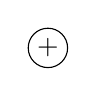
\begin{tikzpicture} \protect \draw (0,0) circle (0.25cm) node at (0,0){+}; \protect \end{tikzpicture}}}
\,abe$\!\!
\protect\raisebox{-2,3mm}{\protect 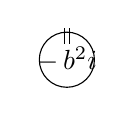
\begin{tikzpicture} \protect \draw (0,0) circle (0.35cm) node at (0,0) {$-\,b^2i$}; \protect \draw (-.03,.2) -- (-.03,.4); \protect \draw (.03,.2) -- (.03,.4); \protect \end{tikzpicture}}%
\!\!
$+\,a^2e + abi - a^2\epsilon, \;$\protect \ovalbox{$+\,abe$}\!
$\protect \raisebox{-2,3mm}{\protect 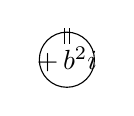
\begin{tikzpicture} \protect \draw (0,0) circle (0.35cm) node at (0,0) {$+\, b^2i$}; \protect \draw (-.03,.2) -- (-.03,.4); \protect \draw (.03,.2) -- (.03,.4); \protect \end{tikzpicture}}
- ab\epsilon \; \sqcap\; 0$
%%%%%%%%%% VAR. 1b
\textit{(b)}~$\displaystyle \frac{ae + bi}{b},$ fiet \mbox{\protect \ovalbox{\textit{abe}} $-\ b^2i$ aequ. $a^2e + b^2i + abi \,+$ \protect \ovalbox{\textit{abe}} $+\, b^2i$},
quia tunc \mbox{$\epsilon \; \sqcap \; 0.$}
\lbrack87~r\textsuperscript{o}\rbrack\
%%%%%%%%%% VAR. 2
\textit{(2)}~Quia ergo % \textit{y} est via centri, ponamus \textit{y} 
\lbrack...\rbrack\ aequ. $\displaystyle \frac{ae - bi}{a + b},$%
~\textit{L}}}
%
at
%
\edtext{aliunde}{%
\lemma{aliunde}\Cfootnote{%
Siehe S.~\refpassage{LH_37_05_086r_aequatioinfall-1}{LH_37_05_086r_aequatioinfall-2}.}}
%
$by^2 +\, a\epsilon^2$ aequ. $ae^2 +\, bi^2.$
Et quia hic
$\epsilon$ aequ. 0,
fiet
\mbox{$by^2 \ \textup{aequ.} \ ae^2+bi^2$}
seu
$y^2$ aequ.
%
\edtext{$\displaystyle \frac{a}{b}e^2 +\, i^2,$
et hoc loco
$y^2$ aequ. $\displaystyle \frac{a^2e^2 - 2abei + b^2i^2}{a^2+2ab+b^2}.$%
}{%
\lemma{$\displaystyle \frac{a}{b}e^2 + i^2,$}\Bfootnote{%
\textit{(1)}~seu $y^2 - i^2$ aequ. $\displaystyle \frac{a}{b}e^2$
\textit{(2)}~et hoc loco
$y^2$ aequ. $\displaystyle \frac{a^2e^2 - 2abei + b^2i^2}{a^2+2ab+b^2}.$%
~\textit{L}}}
%\pend%
%%
%% \footnotesize%
%\pstart%
Ergo fiet:
$a^3e^2 + a^2bi^2 +\, \ovalbox{2}
% \raisebox{-1.5mm}{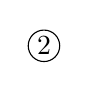
\begin{tikzpicture} \draw (0,0) circle (0.2cm) node at (0,0){2};\end{tikzpicture}}
a^2be^2 +\, 2ab^2i, \, +\, ab^2e^2 \; \ovalbox{$+ \, b^3i^2$} \ \text{aequ.} \ \ovalbox{$a^2be^2$} - 2ab^2ei \; \ovalbox{$+\, b^3i^2$}\,.$%
\rule[-2mm]{0mm}{0mm}%
\pend%
%
% \footnotesize%
\pstart%
Hinc patet
solutionem hoc modo esse impossibilem,%
\protect\index{Sachverzeichnis}{solutio impossibilis}
et perinde corpus,
quod in eam tendit partem cum centro gravitatis%
\protect\index{Sachverzeichnis}{corpus cum centro gravitatis tendens}%
\lbrack,\rbrack\
nec quiescere nec repelli
sed semper progredi post occursum.%
\protect\index{Sachverzeichnis}{occursus}%
\protect\index{Sachverzeichnis}{corpus post occursum progrediens}
Fiat ergo:
via centri gravitatis%
\protect\index{Sachverzeichnis}{via centri gravitatis}%
\protect\index{Sachverzeichnis}{centrum gravitatis}
seu 
\textit{y} aequ. $\displaystyle \frac{bi-a\epsilon}{a+b},$
prodibit idem
et res eodem modo non procedet.%
\rule[-2mm]{0mm}{0mm}%
\pend%
%
% \footnotesize%
\pstart%
Et manifestum est\lbrack:\rbrack\
si corpus occurrens quiescat post occursum,%
\protect\index{Sachverzeichnis}{occursus}%
\protect\index{Sachverzeichnis}{corpus occurrens}%
\protect\index{Sachverzeichnis}{corpus post occursum quiescens}
necessario viam centri gravitatis%
\protect\index{Sachverzeichnis}{via centri gravitatis}
venisse ab ipsius plaga,
quia
corpore altero solo procedente
tendit in adversam plagam.%
\protect\index{Sachverzeichnis}{plaga adversa}
Debet autem distantia esse eadem quae ante.%
\protect\index{Sachverzeichnis}{distantia corporum post concursum}
Ergo corpus excipiens%
\protect\index{Sachverzeichnis}{corpus excipiens}
movebitur celeritate tanta%
\protect\index{Sachverzeichnis}{celeritas corporis excipientis}
quanta antea ambo simul,
at centrum gravitatis%
\protect\index{Sachverzeichnis}{centrum gravitatis}
utique movetur minore%
\protect\index{Sachverzeichnis}{celeritas centri gravitatis}
%
\edtext{quia movetur inter ipsas,}{%
\lemma{quia}\Bfootnote{%
\hspace{-0,5mm}movetur inter ipsas
\textit{erg.~L}}}
%
ergo non possunt esse eaedem,
cum tamen eaedem hoc loco esse debeant;
impossibilis ergo hypothesis%
\protect\index{Sachverzeichnis}{hypothesis quietis}%
\protect\index{Sachverzeichnis}{quies}
\edlabel{LH_37_05_087r_njhe-1}%
quietis.%
%
\edtext{}{%
{\xxref{LH_37_05_087r_njhe-1}{LH_37_05_087r_njhe-2}}%
{%
\lemma{quietis.}\Bfootnote{%
\textit{(1)}~Imo jam
\textit{(2)}~Video%
~\textit{L}}}}
%
\pend%
\vspace{1.0em}
\normalsize%
\pstart%
Video%
\edlabel{LH_37_05_087r_njhe-2}
manifestam conclusionem%
\protect\index{Sachverzeichnis}{conclusio manifesta}
%
\edtext{hanc\lbrack:\rbrack\
si corpus}{%
\lemma{hanc}\Bfootnote{%
\textit{(1)}~corpus
\textit{(2)}~si corpus%
~\textit{L}}}
%
unum tendebat in eandem cum centro gravitatis viam ante concursum,%
\protect\index{Sachverzeichnis}{corpus cum centro gravitatis tendens}%
\protect\index{Sachverzeichnis}{via centri gravitatis}%
\protect\index{Sachverzeichnis}{centrum gravitatis}
alterum tendet in eandem cum eo viam post concursum,%
\protect\index{Sachverzeichnis}{concursus corporum}
semper enim necessario ipsum
%
\edtext{}{{\xxref{KZeitz105}{KZeitz106}}%
{%
\lemma{antecedit.}\Bfootnote{%
\textit{(1)}~Hinc cum via centri ante concursum sit $\displaystyle \frac{ae-bi}{a+b}$
\textit{(2)}~Et cum % distantia corporum 
\lbrack...\rbrack\ maneat eadem,%
~\textit{L}}}}%
\edlabel{KZeitz105}antecedit.
\pend
%
%
%  \newpage% 
  \vspace{2.0em}%	% Diagramm Fig.~3
  \centerline{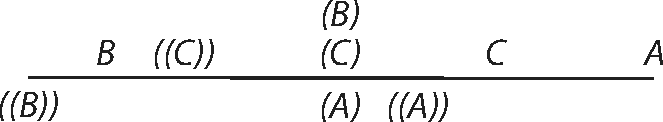
\includegraphics[width=0.48\textwidth]{gesamttex/edit_VIII,3/images/LH_37_05_086-087_d3.pdf}}%
  \vspace{0.5em}
  \centerline{{\normalsize\lbrack\textit{Fig.~3}\rbrack}}%
%  \label{LH_37_05_087r_Fig.3}%
 % \vspace{1.5em}%
 \newpage%
\pstart
Et%
\edlabel{LH_37_05_087r_dkiu-1}
cum distantia corporum maneat eadem,%
\protect\index{Sachverzeichnis}{distantia corporum ante concursum}%
\protect\index{Sachverzeichnis}{distantia corporum post concursum}\edlabel{KZeitz106}%%
%
etiam distantia corporis cujusque a centro gravitatis manebit eadem;%
\protect\index{Sachverzeichnis}{distantia corporum a centro gravitatis}%
\protect\index{Sachverzeichnis}{centrum gravitatis}%
\edlabel{LH_37_05_087r_dkiu-2}
quia eandem semper proportionem habet ad distantiam
corporum,%
\protect\index{Sachverzeichnis}{distantia corporum ante concursum}%
\protect\index{Sachverzeichnis}{distantia corporum post concursum}
eam scilicet
quam corpus oppositum%
\protect\index{Sachverzeichnis}{corpus oppositum}
ad corporum summam.%
\protect\index{Sachverzeichnis}{summa corporum concurrentium}
Eadem autem est quantitas,%
\protect\index{Sachverzeichnis}{quantitas}
cujus ad eandem eadem ratio
\edlabel{LH_37_05_087rlvr-1}%
est.%
%
\edtext{}{%
{\xxref{LH_37_05_087rlvr-1}{LH_37_05_087rlvr-2}}%
{\lemma{est.}\Bfootnote{%
\textit{(1)}~Hinc sequitur corpus quod repellitur
\textit{(2)}~Patet corporis % quod centrum 
\lbrack...\rbrack\ gravitatis antecedit%
~\textit{L}}}}%
%
\pend%
% \newpage%
%
\pstart%
Patet corporis%
\protect\index{Sachverzeichnis}{corpus centrum gravitatis antecedens}%
\protect\index{Sachverzeichnis}{centrum gravitatis}
quod centrum gravitatis antecedit%
\edlabel{LH_37_05_087rlvr-2}
%
viam \textit{(B)((B))} esse aequ.
%
\edtext{\textit{(C)((C))} $+$
[\textit{((C))((B))}].
Inveni tandem}{%
\lemma{\textit{(C)((C))}}\Bfootnote{%
\hspace{-0,5mm} $+$
\textbar~\textit{C((B))} \textit{ändert Hrsg. nach~E, S.~155\cite{01056}}~\textbar.
\textit{(1)}~Corpus id quod
\textit{(2)}~Inveni tandem%
~\textit{L}}}
%
hinc regulam elegantem,%
\protect\index{Sachverzeichnis}{regula elegans}
quando corpus \textit{A}
quod in eandem cum centro gravitatis partem tendit%
\protect\index{Sachverzeichnis}{corpus cum centro gravitatis tendens}%
\protect\index{Sachverzeichnis}{centrum gravitatis}
repellatur vel non.%
\protect\index{Sachverzeichnis}{corpus repulsum}
Repellatur scilicet
quando \textit{AC} majus quam \textit{C(C)},
progreditur quando minus est.%
\protect\index{Sachverzeichnis}{corpus progrediens}
Quod sic demonstro%
\lbrack:\rbrack\
\textit{((A))((C))} aequ. \textit{AC}
(\protect\vphantom)%
\edtext{ut dixi}{%
\lemma{ut dixi}\Cfootnote{%
Vgl.~S.~\refpassage{LH_37_05_087r_dkiu-1}{LH_37_05_087r_dkiu-2}.}}
%
\edtext{eandem distantiam}{%
\lemma{eandem}\Bfootnote{\hspace{-0,5mm}%
\textit{(1)}~est
\textit{(2)}~distantiam%
\textit{L}}}
%
a centro grav. servari%
\protect\index{Sachverzeichnis}{distantia a centro gravitatis servata}%
\protect\index{Sachverzeichnis}{centrum gravitatis}%
\protect\vphantom()
ergo cum \textit{AC} majus quam \textit{C(C)},
etiam \textit{((A))((C))} majus quam \textit{(C)((C))},
adeoque
%
\edtext{\lbrack\textit{((A))}\rbrack}{%
\lemma{\textit{((A))}}\Bfootnote{%
\textit{erg. Hrsg. nach~E, S.~312%
\cite{01056}}}}
%
cadet cis \textit{(C)},
secus est si minus.
Hinc
%
\edtext{patet quomodo}{%
\lemma{patet}\Bfootnote{%
\textit{(1)}~cur non qua
\textit{(2)}~quomodo%
~\textit{L}}}
%
occurrens possit quiescere%
\protect\index{Sachverzeichnis}{corpus post concursum quiescens}%
\lbrack:\rbrack\
nam si \textit{AC} et \textit{C(C)} aequales,
aequabuntur
$\displaystyle \frac{b}{a+b}\;\overline{e+i}$ et $\displaystyle \frac{ae-bi}{a+b},$
sive $be + bi$ et $ae - bi,$
id est 
$be + 2bi$ aequ. \textit{ae}; 
id est
si sit $e + 2i$ ad \textit{e} ut \textit{a} ad \textit{b},
corpus \textit{a}
(\protect\vphantom)%
quod majus est%
\protect\vphantom()
post concursum quiescet.%
\protect\index{Sachverzeichnis}{corpus post concursum quiescens}%
\protect\index{Sachverzeichnis}{concursus corporum}
Repelletur autem%
\protect\index{Sachverzeichnis}{corpus repulsum}
si \textit{AC} majus quam \textit{C(C)},
id est si $b\;\overline{e+i}$ majus quam $ae-bi,$
id est si $\displaystyle \frac{e+2i}{e} \ \groesser \ \displaystyle \frac{a}{b}.$
Progredietur%
\protect\index{Sachverzeichnis}{corpus progrediens}
%
\edtext{vero}{%
\lemma{vero}\Bfootnote{%
\textit{erg.~L}}}
%
si minus
\edlabel{LH_37_05_087rv_rbhk-1}%
sit.
%
\lbrack87~v\textsuperscript{o}\rbrack%  %  %  %  Blatt 87v
%
\edtext{}{%
{\xxref{LH_37_05_087rv_rbhk-1}{LH_37_05_087rv_rbhk-2}}%
{\lemma{sit.}\Bfootnote{%
\hspace{-0,5mm}\lbrack87~v\textsuperscript{o}\rbrack\
\textit{(1)}~Hinc ergo paucis rem omnem sic complector:
quando corpus majus assequitur minus,
tunc post concursum tendunt in easdem partes seu fit
\textit{(a)}~$\displaystyle e + i$ aequ.
\textit{(b)}~\textit{e} $+$
\textit{(c)}~$\displaystyle e + i$ aequ.
\textit{(d)}~\textbar~$e-i$ aequ. $\epsilon + y.$
\textit{streicht Hrsg.}~\textbar\
\textit{(2)}~Quando
\textit{(3)}~Corpora duo \lbrack...\rbrack\ tardius, tunc%
~\textit{L}}}}%
\pend%
 \pstart%
Corpora duo tendunt in easdem partes%
\protect\index{Sachverzeichnis}{corpora in easdem partes tendentia}
et celerius assequitur tardius,%
\protect\index{Sachverzeichnis}{corpus assequens}%
\protect\index{Sachverzeichnis}{corpus celerius}%
\protect\index{Sachverzeichnis}{corpus tardius}
tunc%
\edlabel{LH_37_05_087rv_rbhk-2}
repellitur corpus celerius,%
\protect\index{Sachverzeichnis}{corpus repulsum}
quando \textit{AC} majus quam \textit{C(C)};
est autem \textit{AC} aequ.
$\displaystyle \frac{b}{a+b}\;\overline{e-i}$
et \textit{C(C)} aequ. $e-\displaystyle \frac{be-bi}{a+b}$
seu
%
\edtext{\textit{ae} \protect\ovalbox{$+\, be - be$}\,$-\,bi$}{%
\lemma{\textit{ae} \protect\ovalbox{$+\, be - be$}\,$-\,bi$}\Cfootnote{%
Dem Summanden \textit{bi} kommt das positive Vorzeichen zu;
siehe \textsc{Fichant} 1994, S.~156 u.~313.\cite{01056}
Der Fehler wirkt sich auf die unmittelbar folgenden Herleitungen aus.}}
%
seu $\displaystyle \frac{ae-bi}{a+b},$
%
\edtext{quod si sit minus quam
$\displaystyle \frac{b}{a+b}\;\overline{e-i},$
seu si sit $ae - bi$ minus quam $be - bi,$%
}{%
\lemma{quod}\Bfootnote{%
\hspace{-0,5mm}si
\textbar~sit \textit{erg.}~%
\textbar\ minus
\textbar~quam \textit{erg.}~%
\textbar\ $\displaystyle \frac{b}{a+b}\;\overline{e-i},$ seu si sit
\textit{(1)}~\textit{ae} minus quam
\textit{(2)}~$ae - bi$ minus quam $be - bi,$%
~\textit{L}}}%
\rule[0mm]{0mm}{4mm}
%
seu si sit \textit{ae} minus quam \textit{be},
seu si sit
%
\edtext{\textit{a} minus quam \textit{b},}{%
\lemma{\textit{a} minus quam \textit{b}}\Cfootnote{%
Eigentlich gilt: $\displaystyle a < b\frac{e - 2i}{e}.$
Die Ergebnisse der folgenden Herleitungen sind indessen richtig.}}%
%
\rule[-1mm]{0mm}{5mm}
tunc corpus incurrens repelletur;%
\protect\index{Sachverzeichnis}{corpus repulsum}
sin
%
\edtext{\lbrack majus\rbrack}{%
\lemma{minus}\Bfootnote{%
\textit{L~ändert Hrsg. nach~E, S.~156%
\cite{01056}}}}
%
progredietur.%
\protect\index{Sachverzeichnis}{corpus post concursum progrediens}
\pend%
\newpage
% Diagramm Fig.~4
  \centerline{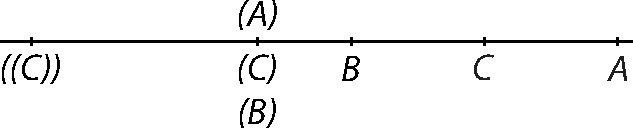
\includegraphics[width=0.48\textwidth]{gesamttex/edit_VIII,3/images/LH_37_05_086-087_d4.pdf}}%\hspace{55mm}
  \vspace{0.5em}
  \centerline{\lbrack\textit{Fig.~4}\rbrack}%\hspace{65mm}
%  \label{LH_37_05_087v_Fig.4}%
  \vspace{2.0em}%
\pstart%
%   !!!   !!!  !!!  !!!   Achtung getrixt:
%
\edtext{}{%
\lemma{\hspace{1,6mm}\lbrack\textit{Fig.~4}\rbrack}\killnumber%
\Cfootnote{Ein ähnliches, weniger vollständiges Diagramm auf Bl.~87~v\textsuperscript{o} wird nicht wiedergegeben.}}%
\edtext{Si \textit{a} repellitur seu}{%
\lemma{Si}\Bfootnote{\hspace{-0,5mm}%
\textit{a} repellitur seu
\textit{erg.~L}}}
%
si \textit{AC} majus quam \textit{C(C)},
erit
$\overset{\displaystyle \phantom{i}\textit{A(C)}}{\displaystyle \frac{b}{a+b}\,\overline{e-i}}$
majus quam
%
$ \underbrace{\underset{\displaystyle e - \frac{b}{a+b}\,\overline{e-i}}{\textit{A(C)} \ - \ AC}}_{\displaystyle\textit{C(C)}},$
%
seu 2\textit{AC}
%
% \raisebox{2.0em}[0.0em][2.0em]{%
majus quam \textit{A(A)}
seu
$\displaystyle\ovalbox{2}\,be - 2bi \ \groesser \ ae\; \ovalbox{$\displaystyle +\, be$}$
%
% $\raisebox{-1.5mm}{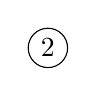
\begin{tikzpicture} \draw (0,0) circle (0.25cm) node at (0,0) {2}; \end{tikzpicture}}\,be - 2bi \ \groesser  \ ab\raisebox{-3.0mm}{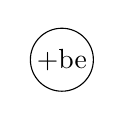
\begin{tikzpicture} \draw (0,0) circle (0.4cm) node at (0,0) {+be}; \end{tikzpicture}}$
seu
$\displaystyle \frac{e-2i}{e} \ \groesser \ \displaystyle \frac{a}{b}.$%
% }%
\rule[-3mm]{0mm}{0mm}
%
\pend%
%
\pstart%
Hinc%
\edlabel{LH_37_05_087v_regula_kdkq-1}
brevius regulam istam colligimus:%
\protect\index{Sachverzeichnis}{regula collecta}%
\rule[-4mm]{0mm}{8mm}
\pend%
%
\pstart%
%\noindent%
Si corpus
quod in eandem cum centro gravitatis partem tendit%
\protect\index{Sachverzeichnis}{corpus cum centro gravitatis tendens}%
\protect\index{Sachverzeichnis}{centrum gravitatis}
sit \textit{a} et ejus celeritas \textit{e},
alterum \textit{b} et
%
\edtext{celeritas ejus%
\protect\index{Sachverzeichnis}{celeritas corporum concurrentium}
\lbrack\textit{i}\rbrack,
\protect\rule[0mm]{0mm}{6mm}%
et corporibus in eandem partem tendentibus sit}{%
\lemma{celeritas}\Bfootnote{%
\hspace{-0,5mm}ejus
\textbar~\textit{e} \textit{ändert Hrsg. nach~E, S.~156\cite{01056}}~\textbar~,
\textit{(1)}~sitque in casu
\textit{(2)}~et corporibus \lbrack...\rbrack\ tendentibus sit%
~\textit{L}}}
%
$\displaystyle \frac{e-2i}{e}$ majus
quam $\displaystyle \frac{a}{b},$
corpus \textit{a} repelletur,%
\protect\index{Sachverzeichnis}{corpus repulsum}
sin minus progredietur,%
\protect\index{Sachverzeichnis}{corpus post concursum progrediens}
si aequalia quiescet.%
\protect\index{Sachverzeichnis}{corpus post concursum quiescens}
\pend%
\pstart%
Iisdem positis
si corpora tendant in partes contrarias%
\protect\index{Sachverzeichnis}{corpora in partes contrarias tendentia}
sitque $\displaystyle \frac{e+2i}{e}$ majus
quam $\displaystyle \frac{a}{b},$
idem continget,%
\rule[-0mm]{0mm}{4mm}
et ita de caeteris.%
\edlabel{LH_37_05_087v_regula_kdkq-2}
\pend%
%
\pstart%
Aequationes ergo%
\protect\index{Sachverzeichnis}{aequatio}
quas habemus
sunt:%
\rule[-2mm]{0mm}{7mm}
\pend%
%
\pstart%
\noindent%
$ae^2 +\, bi^2$ aequ. $a\epsilon^2 +\, by^2,$
%
\edtext{seu $ae^2-a\epsilon^2$ aequ. $by^2-bi^2$}{%
\lemma{seu}\Bfootnote{%
\hspace{-0,5mm}$ae^2-a\epsilon^2$ aequ. $by^2-bi^2$
\textit{erg.~L}}}
%
sive
$\displaystyle \frac{a}{b}$
aequ.
$\displaystyle \frac{y+i,\;y-i}{e+\epsilon,\;e-\epsilon},$
\pend%
%
\pstart%
\noindent%
\raisebox{1.1em}{et} 
% \mbox{%
\begin{tabular}{rcc} 
$\ppmG e\; \ppmH i$ 
& 
aequ.
& 
$(\ppmG\!) \epsilon\, (\ppmH\!) y$
\\ 
$+\, e\; \pleibdashv i$
& 
aequ.
& 
$(\pleibdashv\!)\epsilon\, + y.$ 
\end{tabular}
% }
\pend%
\newpage
\pstart%
Sit \textit{e}
%
\edtext{vel \textit{A(C)}}{%
\lemma{vel}\Bfootnote{\textit{A(C)}
\textit{erg.~L}}}
%
celeritas%
\protect\index{Sachverzeichnis}{celeritas corporum concurrentium}%
\protect\index{Sachverzeichnis}{corpus centrum gravitatis sequens}%
\protect\index{Sachverzeichnis}{centrum gravitatis}
%
\edtext{corporis centrum sequentis,}{%
\lemma{%
corporis}\Bfootnote{%
\textit{(1)}~in eandem cum via centri
\textit{(2)}~centrum sequentis,%
~\textit{L}}}
%
fiet
\mbox{$\overset{\displaystyle e}{A(C)}-AC$} aequ. \textit{C(C)};
est autem \textit{AC} aequ.
$\displaystyle \frac{b}{a+b}\,\overline{\pmG\, e \; \pmH\, i},$
ergo
%
\edtext{\lbrack\textit{C(C)} aequ.\rbrack}{%
\lemma{\textit{C(C)}}\Bfootnote{%
\hspace{-0,5mm}aequ.
\textit{erg. Hrsg. nach E, S.~157%
\cite{01056}}}}
%
$\displaystyle \frac{ae\,\ovalbox{$+\, be \; \pmB\, be$}\; \pmB\, bi}{a+b}.$
Hinc patet:
cum \textit{be} destrui necesse sit,
fore $\ppmG$ aequ. $+$
et $\ppmB$ aequ. $-,$
et $\ppmH$ fieri $\pleibdashv.$
% \pend%
%
% \pstart%
Adeoque fieri:
$\displaystyle \frac{ae\, \leibvdash\, bi}{a+b}$
aequ. \textit{C(C)},
et \textit{AC} aequ.
$\displaystyle \frac{b}{a+b} \, \overline{+\, e\; \leibdashv\, i}.$
\pend%
%
\pstart%
Porro%
\edlabel{LH_37_05_087v_eskfz-1}
post%
\protect\index{Sachverzeichnis}{distantia corporum post concursum}
%
\edtext{concursum distantia est
\lbrack$(\pleibdashv\!)\,\epsilon + y$\rbrack,
quae ante aequ.
\lbrack$+\,e\;\pleibdashv\,i$\rbrack.
Nam}{%
\lemma{concursum}\Bfootnote{%
\textit{(1)}~fit
\textit{(2)}~distantia est
\textbar~$+\,e\;\pleibdashv\,i$ \textit{ändert Hrsg. nach~E, S.~157}\cite{01056}~%
\textbar~, quae ante aequ.
\textbar~$(\pleibdashv\!)\,\epsilon + y$ \textit{ändert Hrsg. nach~E, S.~157}\cite{01056}~%
\textbar~. Nam%
~\textit{L}}}
%
post concursum,%
\protect\index{Sachverzeichnis}{concursus corporum}
sive in easdem tendant partes,%
\protect\index{Sachverzeichnis}{corpora in easdem partes tendentia}
tunc major est celeritas \textit{y},
%
\edtext{ergo ab ea subtrahi}{%
\lemma{ergo}\Bfootnote{%
\textit{(1)}~non addi
\textit{(2)}~ab ea subtrahi%
~\textit{L}}}
%
debet $\epsilon;$
vel in contrarias discedunt,%
\protect\index{Sachverzeichnis}{corpora discedentia in partes contrarias}
tunc inter se addi debent,
tunc non est opus signo $-.$
%\newline%
Ergo semper fiet:
\mbox{$(\pleibdashv\!)\,\epsilon + y$}
distantia corporum post concursum,%
\protect\index{Sachverzeichnis}{distantia corporum post concursum}
posito fuisse
%
\edtext{\lbrack\mbox{$e\; \pleibdashv\: i$\rbrack}}{%
\lemma{$e + i$}\Bfootnote{%
\textit{L~ändert Hrsg.}}}
%
ante concursum.%
\protect\index{Sachverzeichnis}{distantia corporum ante concursum}%
\edlabel{LH_37_05_087v_eskfz-2}
\newline%
Ergo
\mbox{$+\,e\; \pleibdashv\, i$}
aequ.
\mbox{$(\pleibdashv\!)\, \epsilon + y,$}%
\edlabel{LH_37_05_087v_eskfz-3}
\pend%
\vspace{0.75em}%
%
\pstart%
\noindent%
\lbrack\textit{Nachfolgend kleingedruckter Text in L gestrichen:}\rbrack 
\pend%
\vspace{0.5em}%
%
\footnotesize%
\pstart%
\noindent%
$e\; (\pleibvdash\!)\; \epsilon$ aequ. $y\; (\pleibvdash\!)\; i.$
\quad%
\textit{y} aequ. $e\; (\pleibvdash\!)\; \epsilon\; \pleibdashv\; i.$
\quad%
$ae + bi$ aequ. $a\epsilon + by.$
\newline%
Ergo \textit{y} aequ. $\displaystyle \frac{ae + bi - a\epsilon}{b}$
aequ. $e\; (\pleibvdash\!)\; \epsilon\; \pleibdashv\; i.$
\newline%
Ergo $ae + bi - a\epsilon$ aequ. $be\; (\pleibvdash\!)\; b\epsilon\; \pleibdashv\; bi,$
seu $\epsilon$ aequ.
$\displaystyle\frac{ae + bi \; \leibvdash\; bi - be}{a\; (\leibvdash\!)\; b}.$
\newline%
Ergo \textit{y} aequ.
%
$\displaystyle
\frac{\underset{%
\underset{%
\displaystyle \phantom{mmmmmn} \leibdashv\: b^2i\rule[-0,5mm]{0mm}{4mm}}%
{\displaystyle \phantom{mn} -\, abe \phantom{n} - b^2i}}%
{a^2e + abi \; (\leibvdash)\: abe\; (\leibvdash)\: b^2i, +\; b^2e}}{ab + b^2}.
%\underset{%
%\underset{%
%\underset{%
%\displaystyle \overline{\phantom{mm} ab + b^2 \phantom{mm}}}%
%{\displaystyle \phantom{mmmmmn} \leibdashv\: b^2i\rule[-0,5mm]{0mm}{4mm}}}%
%{\displaystyle \phantom{mn} -\, abe \phantom{n} - b^2i}}%
%{a^2e + abi \; (\leibvdash)\: abe\; (\leibvdash)\: b^2i, +\; b^2e}
$
%
%\edtext{%}{%
%\lemma{$\displaystyle \protect\frac{a^2e+abi \protect\underset{\displaystyle -abe}{(\leibvdash)abe}\protect\underset{\displaystyle \protect\underset{\displaystyle \leibdashv b^2 i}{-b^2i}}{(\leibvdash )b^2 i}, +b^2e}{ab+b^2}$}\Bfootnote{\hspace{-0,5mm}%
%\textbar~
%\textit{streicht Hrsg.}~\textbar\ $\epsilon$ aequ.%
%~\textit{L}}}
%
\newline%
\edtext{Rursus \textlangle transigendo\textrangle\ $\epsilon$ ut \textit{y},}{%
\lemma{Rursus}\Bfootnote{%
\hspace{-0,5mm}\textlangle transigendo\textrangle\ $\epsilon$ ut \textit{y},
\textit{streicht Hrsg.}}}
\quad% 
$\epsilon$ aequ.
$\displaystyle \frac{ae + bi - by}{a}$
aequ.
$(\pleibdashv\!)\; e\; (\pleibvdash\!)\; y\; \pleibdashv\; (\pleibdashv\!)\; i.$
\newline%
Ergo $ae + bi - by$ aequ.
%
\edtext{$(\pleibdashv\!)\; ae\; (\pleibvdash\!)\; ay\; \pleibdashv\; (\pleibdashv\!)\; ai.$
\newline%
Ergo \textit{y} aequ.
$\displaystyle \frac{+\; ae + bi\; (\leibvdash)\; ae\; \leibvdash\; (\leibdashv)\; ai}{(\leibvdash)\; a + b}.$ 
$ae + bi$ aequ. $a\epsilon + by.$
$-\; ae\; \pleibdashv\; bi$ aequ. $(\pleibvdash\!)\; \epsilon - by.$
\newline%
Ergo $\displaystyle \frac{\epsilon}{i}$ aequ. $\displaystyle \frac{b}{a},$
vel aequ. 0.
Quorum prius succedit
\normalsize{%
\lbrack\textit{Text bricht ab.}%
}\rbrack}{%
\lemma{$(\pleibdashv\!)\; ae\; (\pleibvdash\!)\; ay\; \pleibdashv\; (\pleibdashv\!)\; ai.$}\Bfootnote{%
\hspace{-0,5mm}Ergo \lbrack...\rbrack\ prius succedit
\textit{streicht Hrsg.}}}%
%
\pend%
\newpage
%\vspace{1.0em}
%
\normalsize%
\pstart%
\noindent%
seu
$e\; (\pleibvdash\!)\; \epsilon$
aequ.
$y\; \pleibvdash\, i,$
et \textit{y}
aequ.
$e\; (\pleibvdash\!)\; \epsilon\; \pleibdashv\, i,$
\newline%
et fiet via centri post concursum%
\protect\index{Sachverzeichnis}{via centri gravitatis post concursum}%
\protect\index{Sachverzeichnis}{centrum gravitatis}
$\displaystyle \frac{by\; (\leibvdash)\; a\epsilon}{a + b}$
aequ. \textit{(C)((C))},
\newline%
adeoque habebitur aequatio%
\protect\index{Sachverzeichnis}{aequatio}
$ae\; \pleibvdash\: bi$ aequ. $by\; (\pleibvdash\!)\; a\epsilon,$
\newline%
seu 
$ae\; (\pleibdashv\!)\; a\epsilon$ aequ. $by\; \pleibdashv\, bi;$
\newline%
multiplicetur per 
$e\; (\pleibvdash\!)\; \epsilon$ aequ. $y\; \pleibvdash\, i,$
\newline%
fiet:%
\rule[0mm]{0mm}{2,0mm}
$ae^2 - a\epsilon^2$ aequ. $by^2 - bi^2;$
\newline%
addamus invicem:%
\rule[0mm]{0mm}{4,5mm}
$\underset{\displaystyle +\, ae\; (\leibvdash)\; a\epsilon}{+\, ae\; (\leibdashv)\; a\epsilon}$
aequ.
$\underset{\displaystyle ay\; \leibvdash\; ai}{by\ \leibdashv\ bi}$
\newline%
fiet:%
\rule[0mm]{0mm}{4,5mm}
2\textit{ae} aequ.
$\overline{\vphantom{\leibvdash} a + b}\: y ,\!,\; \overline{\,\leibdashv\; b\: \leibvdash\; a}\: i,$
\newline%
et%
\rule[0mm]{0mm}{5,5mm}
$(\pleibdashv\!)\,
\edtext{\lbrack2ae\rbrack}{\lemma{$2a\epsilon$}\Bfootnote{\textit{L~ändert Hrsg.}}}$
aequ.
$\underset{\displaystyle -\, a\protect\vphantom{H}}{\overline{+\, b\vphantom{\leibvdash}}}\; y\ \; \underset{\displaystyle \phantom{H}a}{\overline{\,\leibdashv\; b}}\: i.$
\pend%
%
\pstart%
Ut
%
\edtext{inveniamus \lbrack signa\rbrack\ \lbrack$\,\pleibdashv$\rbrack\ et $(\pleibdashv\!),$}{%
\lemma{inveniamus}\Bfootnote{% \hspace{-0,5mm}%
\textit{(1)}~signa
\textit{(a)}~$\pleibvdash$
\textit{(b)}~$\pleibdashv$ 
\textit{(2)}~\textbar~signum \textit{ändert Hrsg.}
\textbar~$\pleibdashv$ \textit{erg. Hrsg.}~%
\textbar\ et $(\pleibdashv\!)$,%
~\textit{L}}}
%
tractabimus illa instar incognitarum.%
\protect\index{Sachverzeichnis}{incognita}%
\protect\index{Sachverzeichnis}{signum}%
\rule[0mm]{0mm}{4,5mm}
Vocemus 
$\pleibdashv\, f$
et
$(\pleibdashv\!)\, g.$
Prodibunt aequationes:
$e + fi$ aequ. $g\epsilon + y,$
et $by - ga\epsilon$ aequ.
%
\edtext{$ae - fbi.$
Ut ergo inveniamus \textit{g} ex dato \textit{f},
fiet ex priori aequatione%
\protect\index{Sachverzeichnis}{aequatio}%
\protect\rule[0mm]{0mm}{3,0mm}
$ga\epsilon$ aequ. $ae + fai - ay,$ 
et ex posteriori 
$by + fbi - ae.$}{%
\lemma{$ae - fbi.$}\Bfootnote{%
\textit{(1)}~Ex priori fiet
\textit{(a)}~$ga\epsilon$
\textit{(b)}~\textit{fbi} aequ. \mbox{$gb\epsilon + by - be$}
\textit{(2)}~Ex priori fiet:
\textit{(3)}~Ut ergo % inveniamus \textit{g} ex 
\lbrack...\rbrack\ dato \textit{f}
\textit{(a)}~fiet $ga\epsilon$ aeq
\textit{(b)}~fiet ex priori \lbrack...\rbrack\ posteriori $by + fbi - ae.$%
~\textit{L}}}
%
Ergo fiet:%
\rule[0mm]{0mm}{6,0mm}
$\displaystyle\frac{2ae - ay - by}{bi - ai}$
aequ. \textit{f}.
Sed quia solius tantum \textit{g} valorem quaerimus%
\protect\index{Sachverzeichnis}{valor quaesitus}
sine \textit{y} et $\epsilon,$
sic procedere licebit ope duarum aequationum%
\protect\index{Sachverzeichnis}{aequatio}%
\rule[0mm]{0mm}{4,0mm}%
\lbrack:\rbrack\ 
\textit{y} aequ.
$e + fi - g\epsilon,$ 
et rursus 
\textit{y} aequ.
%
\edtext{$\displaystyle \frac{ae - fbi + ga\epsilon}{b};$%
\protect\rule[0mm]{0mm}{6,0mm}
ergo $ga\epsilon + gb\epsilon$
aequ. $be + fbi - ae + fbi,$}{%
\lemma{$\displaystyle \protect \frac{ae-fbi+ga\epsilon}{b};$}\Bfootnote{%
\textit{(1)}~ergo \protect $2ga\epsilon$ aequ. $ae + fai - ae + fbi$
\textit{(2)}~ergo $ga\epsilon+gb\epsilon$ aequ. $be + fbi - ae + fbi,$%
~\textit{L}}}
%
seu $g\epsilon$ aequ. $\displaystyle\frac{be + 2fbi - ae}{a + b}.$
Ergo%
\edlabel{LH_37_05_087v_regula_afnj-1}
si $be + 2fbi$ majus quam \textit{ae},
vel si $\displaystyle \frac{e\; \leibdashv\; 2i}{e}$
majus quam $\displaystyle \frac{a}{b},$
\textit{g} erit $+$
seu corpus \textit{a} repelletur,%
\protect\index{Sachverzeichnis}{corpus repulsum}
sin minus progredietur,%
\protect\index{Sachverzeichnis}{corpus post concursum progrediens}
si aequalia sint quiescet.%
\protect\index{Sachverzeichnis}{corpus post concursum quiescens}%
\edlabel{LH_37_05_087v_regula_afnj-2}%
\rule[0mm]{0mm}{5,5mm}
Atque ita ex solo calculo%
\protect\index{Sachverzeichnis}{calculus}
cuncta absolvimus.%
\rule[0mm]{0mm}{5,5mm}
Demonstranda superest regula%
\protect\index{Sachverzeichnis}{regula centri gravitatis}%
\protect\index{Sachverzeichnis}{regula distantiae}
vel centri%
\protect\index{Sachverzeichnis}{centrum gravitatis}
vel distantiae.%
\protect\index{Sachverzeichnis}{distantia corporum concurrentium}
\pend%
\count\Bfootins=1200%
\count\Afootins=1200%
\count\Cfootins=1200
%%
%\pstart%
%??? Tentandum an
%\pend%
%%
%\pstart%
%Scheda nona
%\pend
%
%
% Ende des Textes auf Blatt 87v
%
%